\documentclass[a4paper,11pt]{article}

\usepackage[top=1in, bottom=1in, left=1in, right=1in]{geometry}

\usepackage{floatrow}
\usepackage{algorithm}
\usepackage{algorithmic}
\usepackage{subfigure} 
\usepackage{amssymb}
\usepackage{amsmath}
\usepackage{booktabs}
\usepackage{graphicx}
\usepackage{url}

\newcommand{\argmin}{\operatornamewithlimits{argmin}}


\begin{document}

\noindent{\Huge Supplementary Information}


\section{Optimization algorithm}

\begin{algorithm}[!h]   \caption{Alternating Least Squares}
   \label{alg}
   %\begin{minipage}{0.9\textwidth}
   \begin{small}
\begin{algorithmic}[1]
\STATE \textbf{Input}: \\
$k$ : number of latent factors\\
$\Gamma$: pairs of entities for initialization\\
For every task $t$,\\
${\{\mathbf{x}_{ti}\}, \{\mathbf{y}_{tj}\}}$: feature vectors for pathogen and host proteins resp.\\
$\Omega_t$: the observed entries of the matrix $M_t$\\
\STATE \textbf{Initialization}: \\
\STATE An iteration $r$, let $\mathbf{S}^r$ represent $\{S^r_t\}_{t=1}^T$
\STATE $\mathbf{S}^0 \leftarrow 0$
\STATE $U^0 \leftarrow$ top-$k$ left singular vectors and $V^0 \leftarrow$ top-$k$ right singular vectors from the SVD of $\displaystyle{\sum_{(i,j) \in \Gamma}} \mathbf{x}_i \mathbf{y}_j^\intercal$\\
\STATE $\mathcal{L}^0$ : initial loss
\REPEAT
  \STATE $U^{r+1} \leftarrow \displaystyle{\argmin_{U}} \; \mathcal{L}(U, V^r, \mathbf{S}^r)$  \STATE $V^{r+1} \leftarrow \displaystyle{\argmin_{V}} \; \mathcal{L}(U^{r+1}, V, \mathbf{S}^r) $  \STATE For each task $t$\\
  \hspace{0.5cm} $S^{r+1}_t \leftarrow \displaystyle{\argmin_{S_t}} \; \mathcal{L}(U^{r+1}, V^{r+1}, \mathbf{S}^r_{-t}) $
  \STATE Compute $\mathcal{L}^{r+1}$ and let $\delta \leftarrow (\mathcal{L}^r - \mathcal{L}^{r+1})/\mathcal{L}^r$
\UNTIL {$\delta < \tau$}%\While
\end{algorithmic}\end{small}
%\end{minipage}
\end{algorithm}


\section{Parameter tuning}
We tune the hyper parameters using a 3 fold cross-validation (CV) on the training split. For all baseline regularization parameters %(or a grid search based on the method): 
we tried the range: [$100, 50, 10, 1, 0.1, 0.01, 0.05, 10^{-3}$]. To address the class-skew we 
assign a higher weight to the positives. For BSL-MTL, to tune the rank parameter '$k$' we tried: [1, 5, 10, 25, 40, 60, 100] and the regularization parameter controlling the norm of $U$ and $V$ was tuned over the range $\lambda$=$\{1 ... 10^{-3}\}$. For each task $t$, $\sigma_t$ was varied over the values $[10^{-3}, 10^{-4}, 10^{-5}, 10^{-6}]$ and
$\mu_t$ was varied over $\{0, 0.25, 0.5, 0.75, 1\}$.
The optimal setting was:  $k=10$. %, $\lambda = 0.01$, $\sigma_{ebola}=10^{-5}$, $\sigma_{flu}=\sigma_{hepc}=10^{-6}$.

%\subsection{Disadvantages of the Homolog method}
%In Figure \ref{fig:network} we show for each task, the protein interactions in the test data (for one train-test split) that were not found by the homologs model which relies purely on homology-based sequence similarity. The interactions mainly involve human proteins which do not have a homolog in the training data. This illustrates that our features capture more information than mere sequence similarity. Further, inclusion of interactions from other viruses in the na\"ive manner as done by the homologs in fact hurts the performance (results in too many false positives) - our model is able to learn what to borrow from the other tasks accurately.



%\begin{figure}
%\begin{tabular}{c}
%%\begin{minipage}{0.3\textwidth}
%%\begin{center}
%%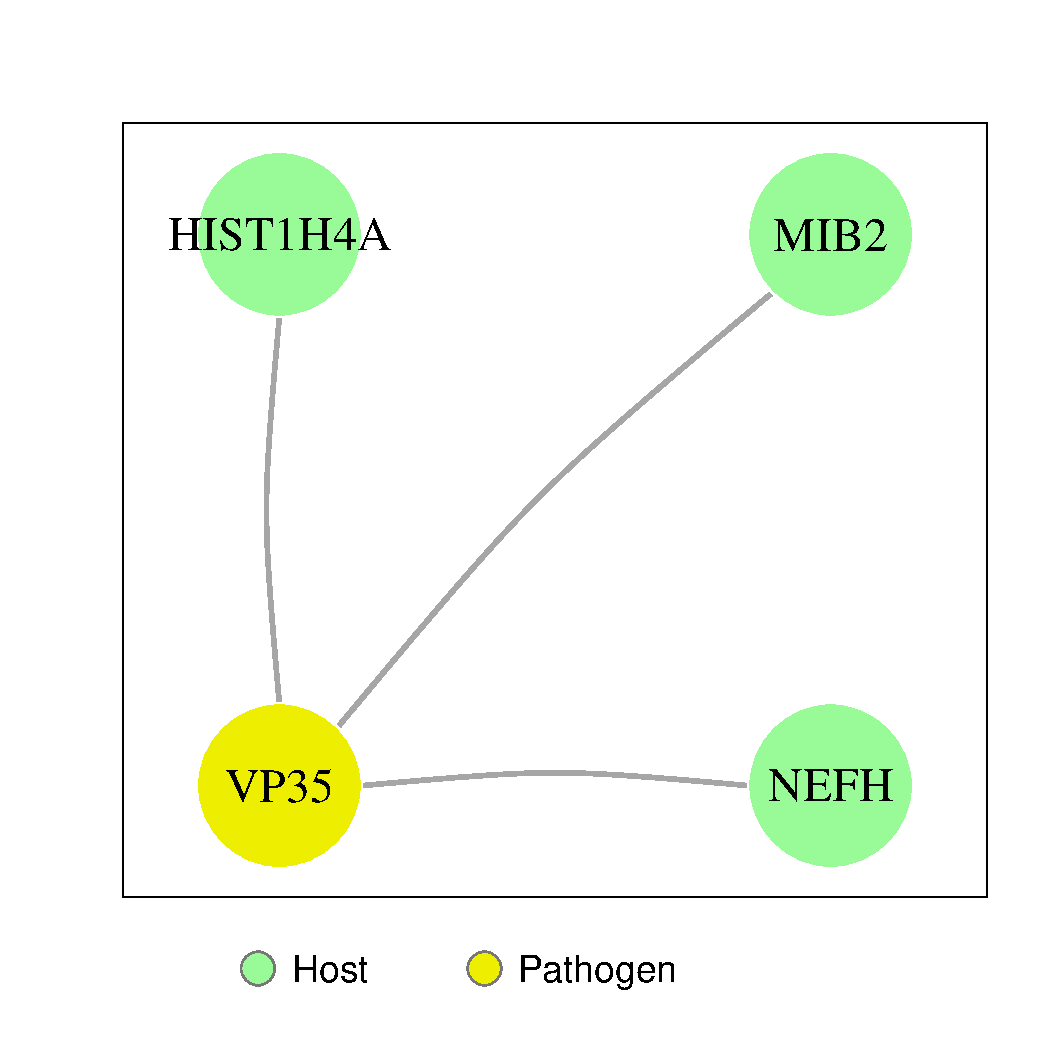
\includegraphics[scale=0.23, trim = 0.3 0 0.2 0.2]{ebolanet.pdf}\vspace{0.6cm}
%%\end{center}
%%\end{minipage}
%%&
%\begin{minipage}{0.4\textwidth}
%\begin{center}
%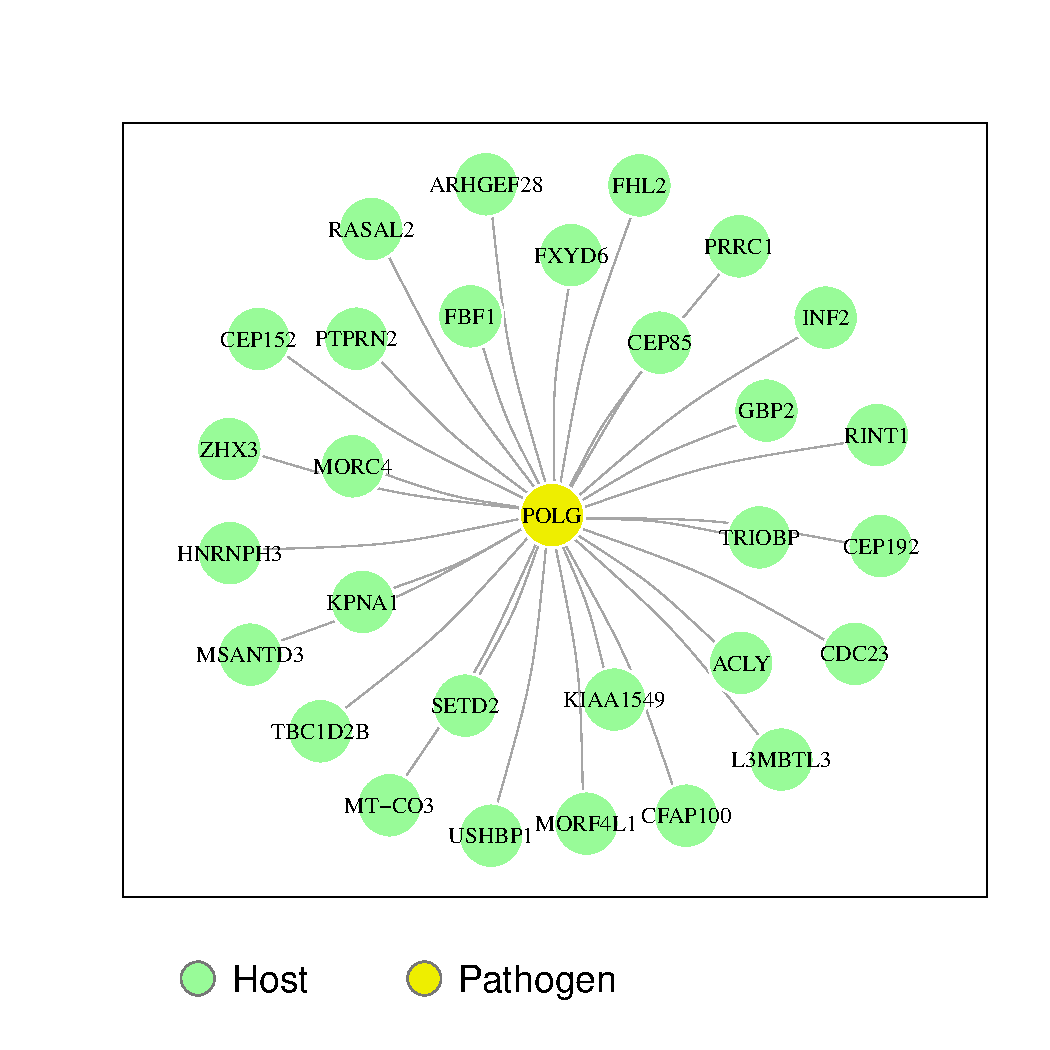
\includegraphics[scale=0.25, trim = 0.7cm 0.7cm 0.7cm 0.7cm]{flavinet.pdf}
%\end{center}
%\end{minipage}
%\\
%\begin{minipage}{0.4\textwidth}
%\begin{center}
%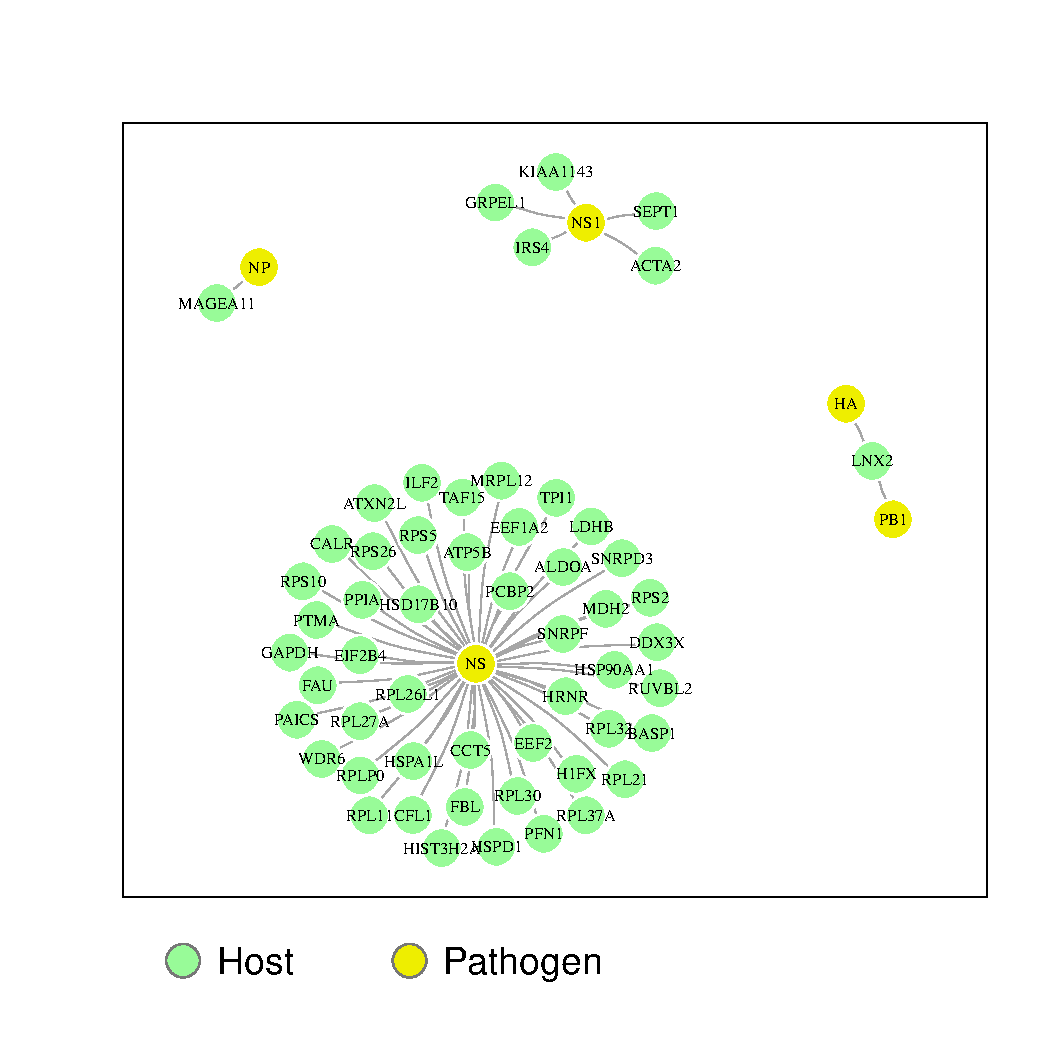
\includegraphics[scale=0.25, trim = 0.5cm 0.5cm 0.5cm 0.5cm]{flunet.pdf}
%\end{center}
%\end{minipage}
%\end{tabular}
%\caption{PPI from each task that are found by our method but are missed by the homolog method. To obtain these, we chose a random train/test split and picked examples from the test data on which the homolog method fails - these are ones for which sequence-similar proteins are not found. (a) shows \textit{Ebola}-human PPI, (b) \textit{Hepatitis-C} human PPI and (c) \textit{Influenza}-human PPI.}
%\label{fig:network}
%\end{figure}



\section{Biological significance of interactions} 

We analyze sequence motifs derived from the top $k$-mers that contribute to interactions. The significant entries of the model parameters $U$, $V$ and $\{S_t\}$ were used to
compute these motifs. The top positive-valued entries from the product $U V^T$ indicate which pairs of features: ($(f_v, f_h)$: virus protein feature, human protein feature) are important for interactions across all the virus-human PPI tasks.
Analogously, the entries from $S_t$ give us pairs of features important to a particular virus-human task `$t$'.
We find that most of the top entries from $U V^T$ correspond to linear virus features, whereas those from the various $S_t$
involve bilinear features. 

We analyze the $k$-mers corresponding to the top 20 features from each of the matrices.

Note that our features do not directly correspond to a unique amino-acid $k$-mer (see Section 4.2):
the virus feature $f_v$ will map to several amino-acid sequences (for instance KKCC, KRCC, RRCC etc all map to a single feature due to the molecular similarity between the amino acids K and R being both positively charged). Given the set of top virus features we can obtain the corresponding set of
amino-acid $k$-mers, say $AA_v$, by reversing the feature-generation step. However most of the possible $k$-mers do not appear in the
training data (ex: out of the 160,000 (=$20^4$) possible 4-mers $\approx$24,000 appear). Let $AA_{tr}$
be the set of amino-acid k-mers that appear in the training data. Then, the intersection $I_v = AA_v \cap AA_{tr}$ gives us the important amino-acid $k$-mers from virus proteins w.r.t interaction prediction.
To summarize $I_v$, we use a popular tool Seq2Logo to generate a sequence motif.
The logos for the two-, three-, four-mers from $I_v$ are generated independently. Since we only
want to summarize, we use the Shannon logo type (which does not consider any background amino-acid distribution)
with the following settings: clustering-method=None, weight-on-prior=1 (pseudo-counts do not make sense in our
analysis). Figure \ref{fig:virus_motifs} shows the motif that is common across viruses. %, while the other figures highlight those motifs important in a specific species.
We observe that the shared tri-mer motif for virus proteins in Figure \ref{fig:virus_motifs} is dominated by
hydrophilic amino acids (T, K, R, D, E).

This procedure described above is used to analyze the most significant human protein features, obtained from
the matrix $U V^T$. These motifs are shown in the supplementary. The task-specific features i.e significant $k$-mers from virus-proteins of \textit{Ebola}, \textit{Hepatitis} and \textit{Influenza} are obtained from the matrices $S_{ebola}$, $S_{hepc}$ and $S_{flu}$ respectively. The motif for Hepatitis is shown in Figure \ref{fig:virus_motifs}(right); the rest can be found in the supplementary. %Knowledge of these pathogen-specific $k$-mers can help in design of drugs to target specific pathogens. These are shown in Figures \ref{fig:ebola_motifs}, \ref{fig:hepc_motifs} and \ref{fig:flu_motifs}.
The virus-specific motifs seem to be dominated by hydrophobic residues (I, P, L, V, A, G) though S and T do appear in some motifs as well.
%The human protein motifs are shown in \ref{fig:human_motifs}; the 3-mer motif show less of a pattern, in particular the first residue does not seem to have any dominant amino-acids.
%However the 4-mer seems to be dominated by hydrophobic amino-acids L, P, I, F in the first three positions and hydrophilic residues S, T, Y in the fourth.
%The human protein motifs are shown in Fig \ref{fig:human_motifs}. In most cases, the first position of the tri-mer was less significant than the second and third, while for the tetramer all four positions show clear preferences.

%The motifs for tri-mers are shown in the supplementary.



 \noindent\emph{Phosphorylation sites}: 
 We found the frequent occurrence of S and T and sometimes Y in the motifs striking and suspected this may be
 related to the amino acids being frequent targets of phosphorylation.
 Phosphorylated sites often serve as PPI sites, and databases such as Phosphosite are
  repositories for known sites in human proteins. Since these are sites in human proteins, we searched for the patterns
	from the 4-mer motif in Fig \ref{fig:human_motifs} and found several to be flanking known phosphorylation sites in human proteins:
	\texttt{LLLs}, \texttt{LLLt}, \texttt{ILLs}, \texttt{PPPs}, \texttt{PIPs}, \texttt{PIPt}, \texttt{LIPs}, \texttt{PLLt} (lower-case indicates the putative phosphorylation site). This observation also supports the notion that the motifs predictive
	of interaction are biologically significant.

\noindent\emph{Evidence in IEDB}\footnote{\url{www.iedb.org}}:
We found experimental evidence for the significance for the virus motifs in the Immune Epitope\footnote{An epitope is a very short sequence from the virus that binds to human antibodies} database (IEDB).
The pattern \texttt{IVGG} from the \textit{Hepatitis-C} motif in Fig. \ref{fig:hepc_motifs} is found in 53 epitopes.
From the \textit{Ebola} motifs in Fig \ref{fig:ebola_motifs}, we find that \texttt{TLAT} is part of six different epitopes, \texttt{SLTT} appears in three epitopes. \texttt{PLIK}, \texttt{SLLL} from the \textit{Influenza} motif are also found in many epitopes.
Finding that the virus k-mer patterns predicted by our method are recognized by human antibodies
is a further validation of its performance.
Further, using higher dimensional $k$-mers (where $k$=7, 8, 9) as
features in our model will give motifs from which complete epitopes can be derived. % which can then be verified by biochemical peptide interaction assays.
Our model thus has applications in epitope prediction as well, where conventional methods consist of scanning all possible $k$-mers from protein sequences to identify likely epitopes.


\begin{figure}
%trim option's parameter order: left bottom right top
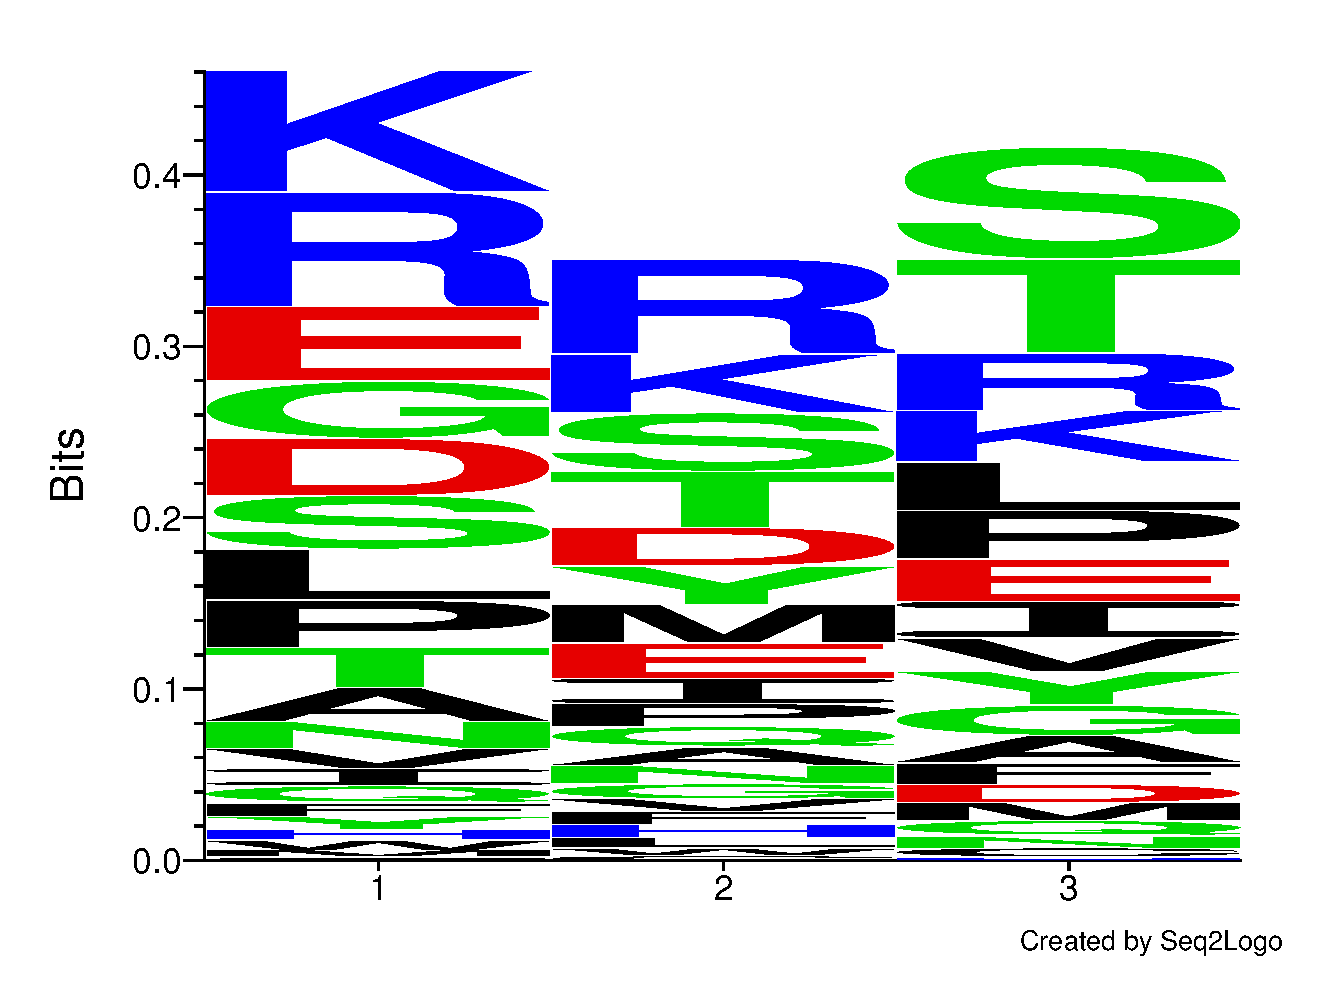
\includegraphics[scale=0.165, trim = 0 0.8cm 0 0]{fig4-eps-converted-to.pdf}
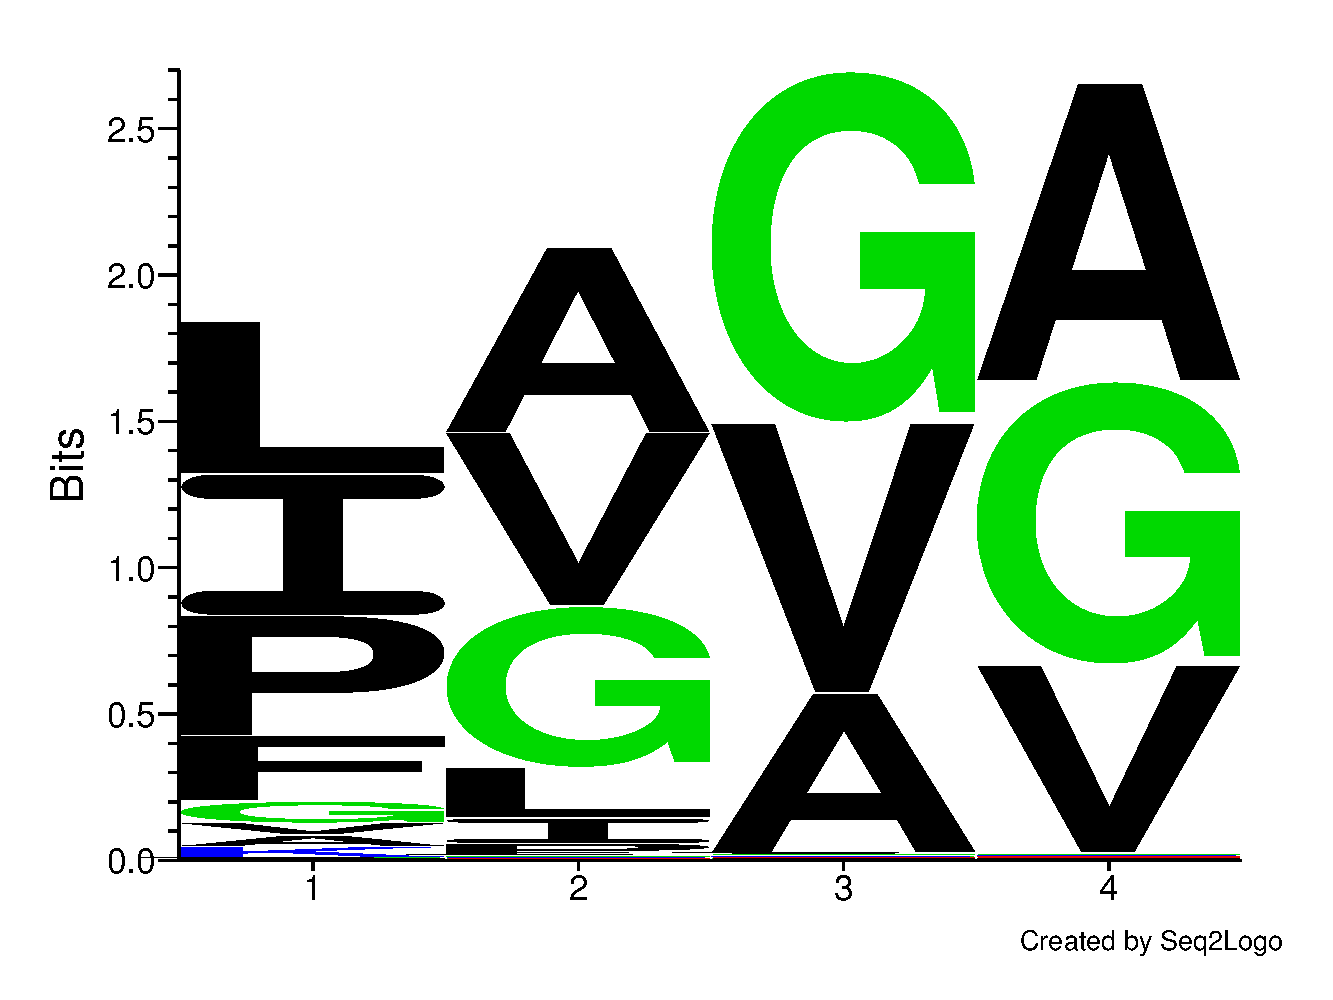
\includegraphics[scale=0.165, trim = 0 0 0 0]{fig8-eps-converted-to.pdf}
\caption{(\textit{Left}) Top tri-mer sequence motifs from virus proteins across all three viruses. These correspond to features important for interactions and is derived from our model parameter $H = U V^{T}$. (\textit{Right}) Motif corresponding to enriched 4-mer patterns found by our model (parameter: $S_{hepc}$) for the Hepatitis-C virus task.}%
\label{fig:virus_motifs}
\end{figure}


\begin{figure}[h]
\begin{floatrow}
\ffigbox[0.45\columnwidth]{%
%trim option's parameter order: left bottom right top
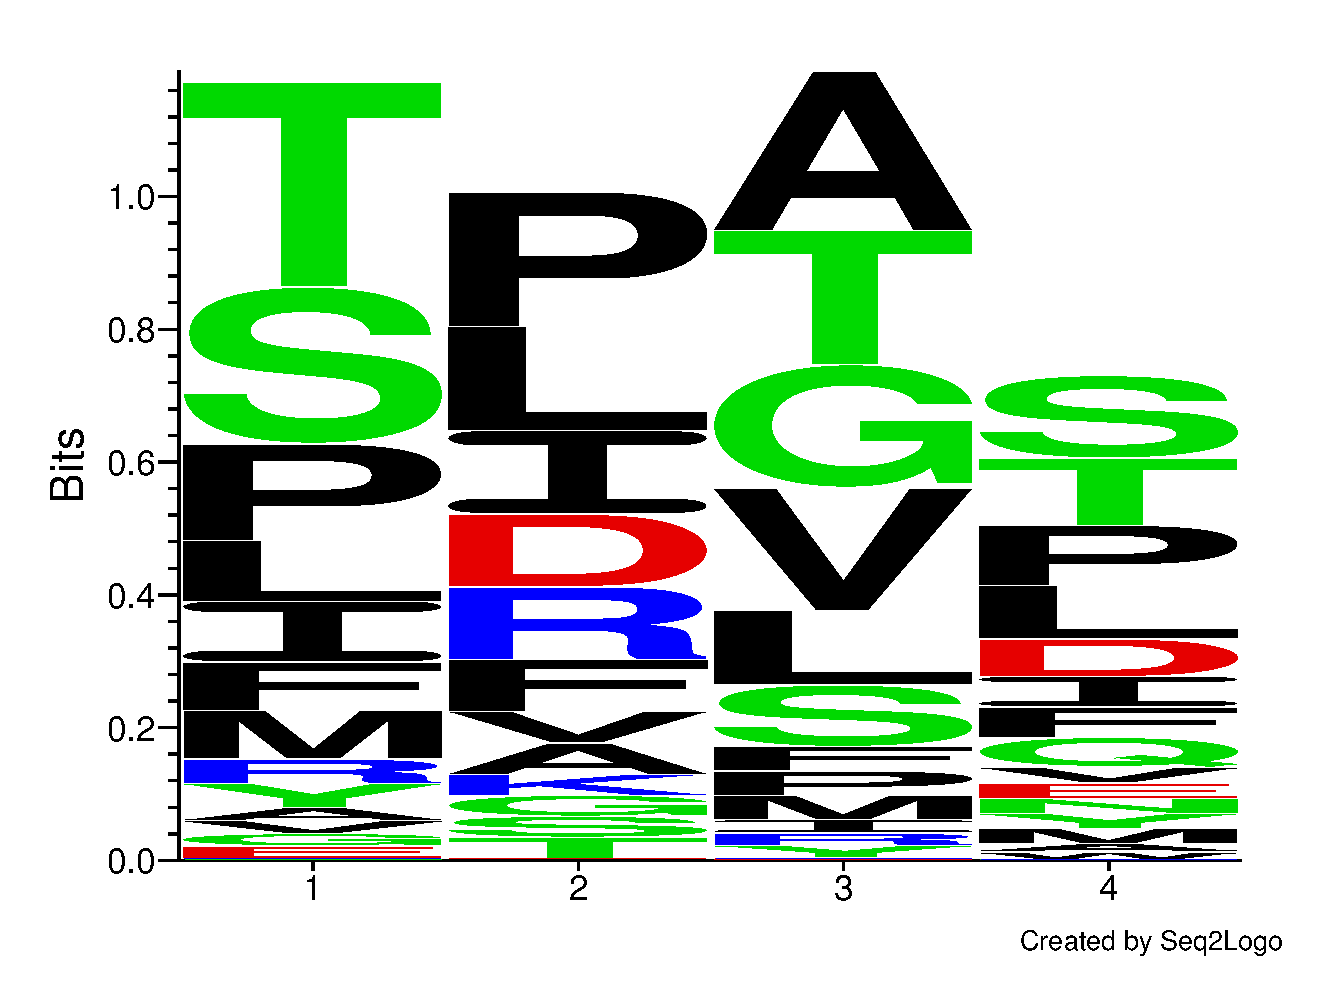
\includegraphics[scale=0.25, trim = 0.2cm 0 0 0]{fig7-eps-converted-to.pdf}
}{%
\caption{Sequence motif from top four-mer features specific to \textit{Ebola} proteins}%
\label{fig:ebola_motifs}
}

\ffigbox[0.45\columnwidth]{%
%trim option's parameter order: left bottom right top
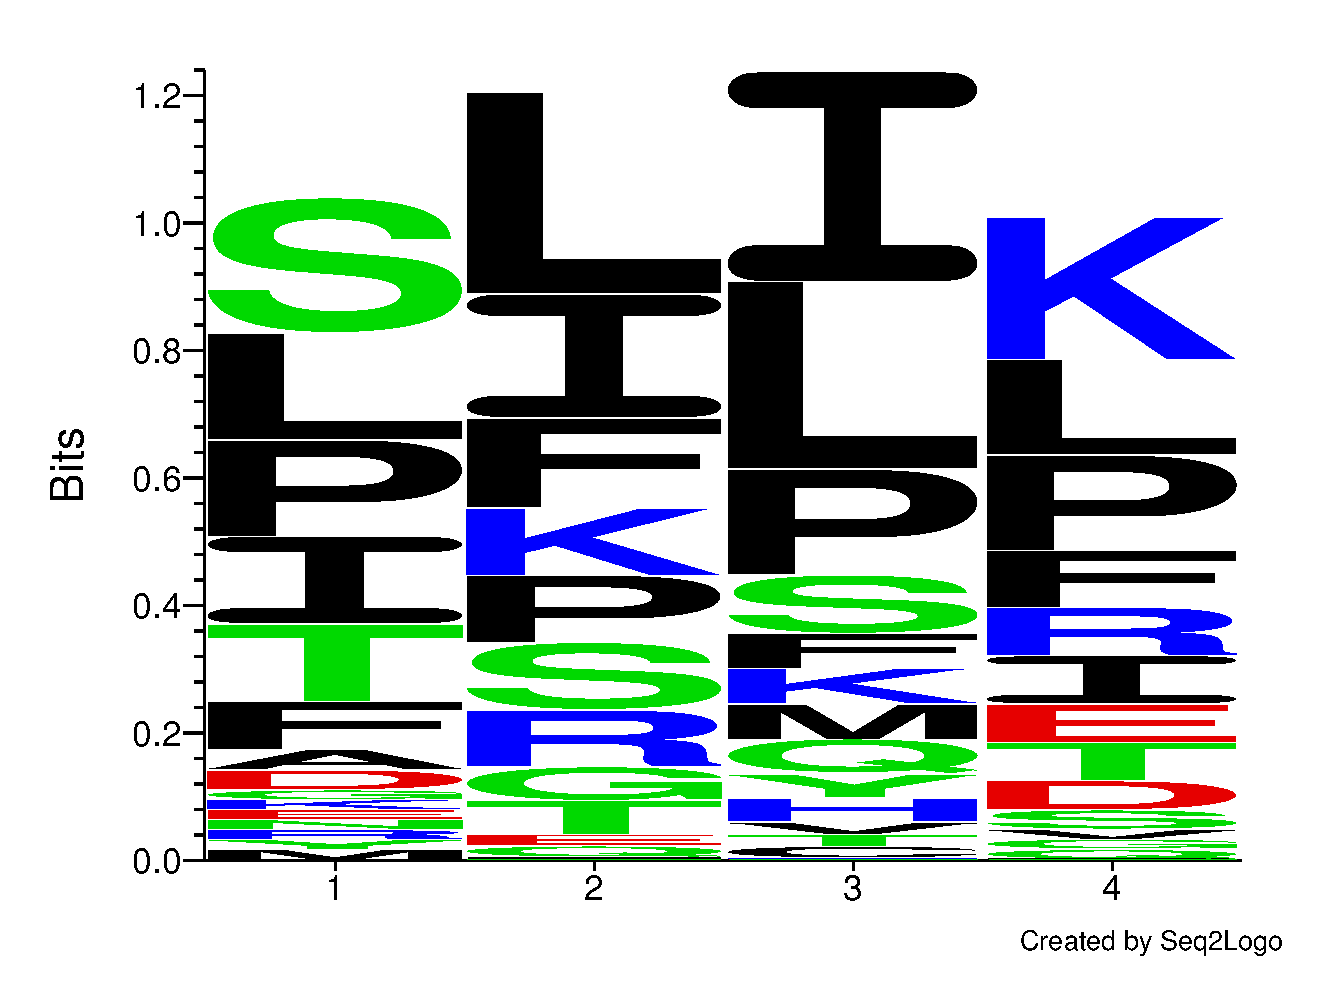
\includegraphics[scale=0.25, trim = 0 0 0 0]{fig9-eps-converted-to.pdf}
}{%
\caption{Sequence motifs specific to \textit{Influenza} proteins that are also important to interactions.}%
\label{fig:flu_motifs}
}


\end{floatrow}
\end{figure}


\section{Tri-mers}

Below, we show the sequence motifs from the tri-mers found to be highly relevant to predicting interactions between human and viral proteins.

\begin{figure}[h]
\begin{floatrow}
\ffigbox[0.45\columnwidth]{%
%trim option's parameter order: left bottom right top
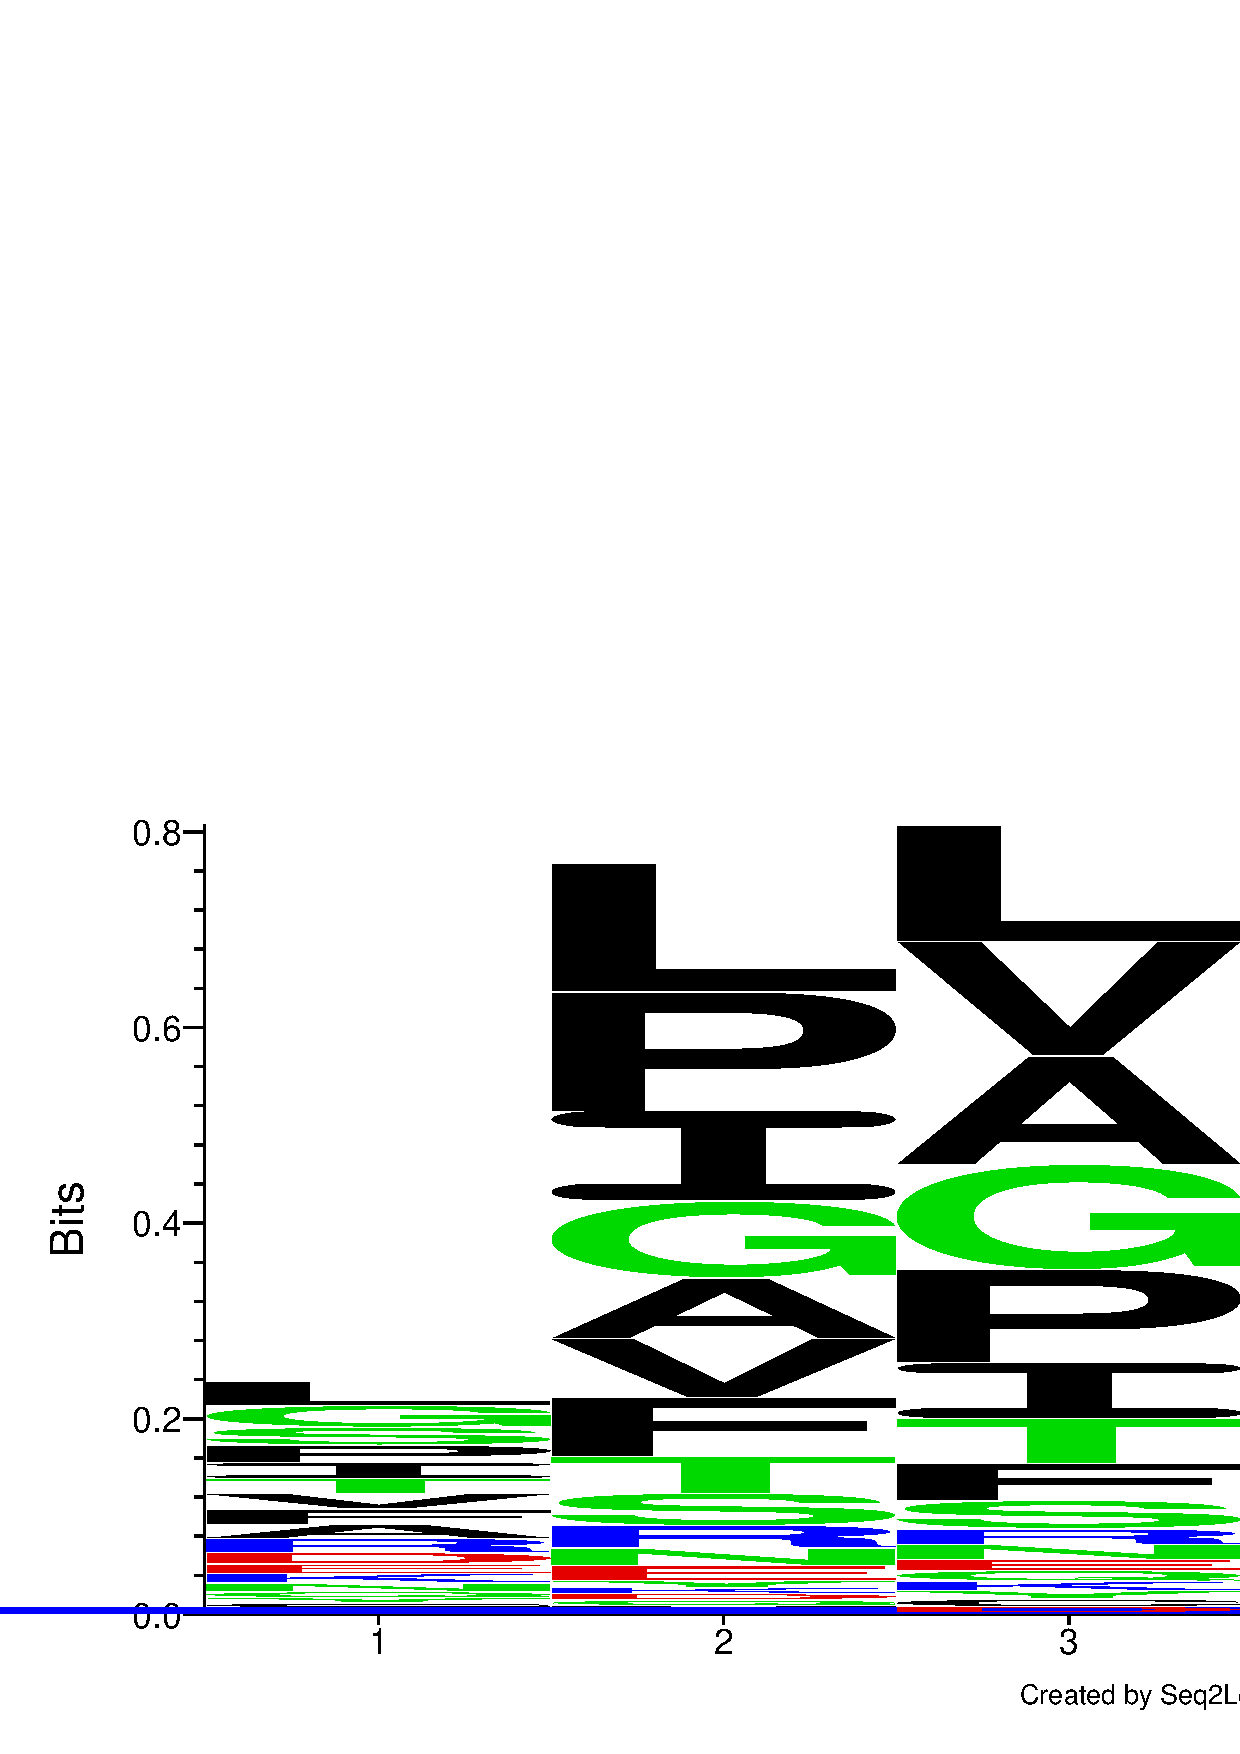
\includegraphics[scale=0.25, trim = 0 0 0 0]{top10flavi_3mers_seq2logo.pdf}
}{%
\caption{Sequence motifs specific to \textit{Hepatitic-C} proteins that are also important to interactions.}%
\label{fig:hepc_motifs}
}
\ffigbox[0.45\columnwidth]{%
%trim option's parameter order: left bottom right top
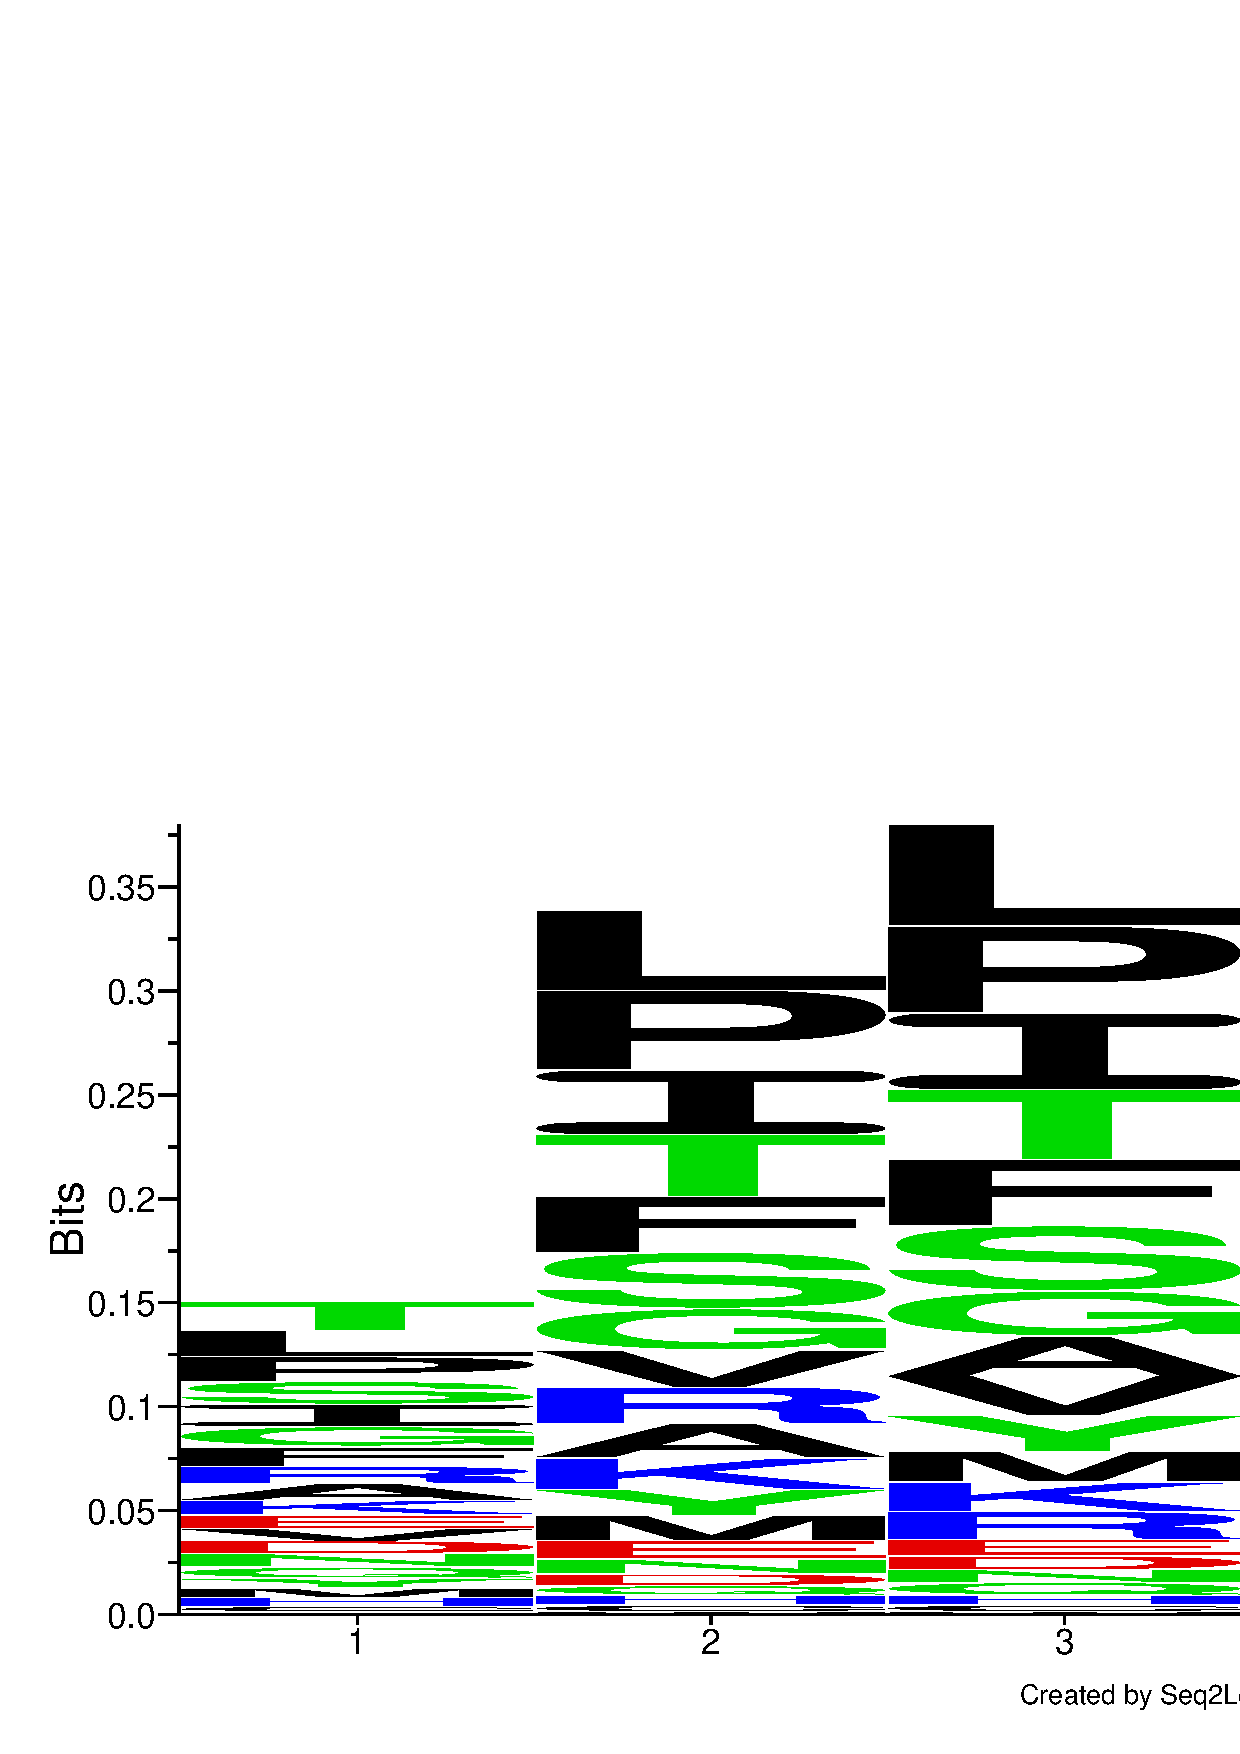
\includegraphics[scale=0.25, trim = 0 0 0 0]{top10human_3mers_seq2logo.pdf}
}{%
\caption{Sequence motif constructed from the top tri-mer features of human proteins}%
\label{fig:human_motifs}
}
\end{floatrow}
\end{figure}

%\bibliographystyle{plain}
%\bibliography{references}

\end{document}
